\documentclass[english,hidelinks, 11 pt, class=report,crop=false]{standalone}
\newcommand{\texandasy}{Teksten er skrevet i \LaTeX\ og figurene er lagd ved hjelp av Asymptote.}

\newcommand{\expl}{forklaring}

\newcommand{\note}{Merk}
\newcommand{\notesm}[1]{{\footnotesize \textsl{\note:} #1}}
\newcommand{\ekstitle}{Eksempel }
\newcommand{\sprtitle}{Språkboksen}
\newcommand{\vedlegg}[1]{\refstepcounter{vedl}\section*{Vedlegg \thevedl: #1}  \setcounter{vedleq}{0}}

\newcommand\sv{\vsk \textbf{Svar} \vspace{4 pt}\\}

% exercises
\newcommand{\opgt}{\newpage \phantomsection \addcontentsline{toc}{section}{Oppgaver} \section*{Oppgaver for kapittel \thechapter}\vs \setcounter{section}{1}}

\newcommand{\grubop}[1]{\vspace{15pt} \refstepcounter{grub}\large \textbf{\color{blue} Gruble \thegrub} \vspace{2 pt} \label{#1} \\}
\newcommand{\grubr}[1]{\vspace{3pt}\textbf{Gruble \ref{#1}}}

%references
\newcommand{\reftab}[1]{\hrs{#1}{tabell}}
\newcommand{\rref}[1]{\hrs{#1}{regel}}
\newcommand{\dref}[1]{\hrs{#1}{definisjon}}
\newcommand{\refkap}[1]{\hrs{#1}{kapittel}}
\newcommand{\refsec}[1]{\hrs{#1}{seksjon}}
\newcommand{\refdsec}[1]{\hrs{#1}{delseksjon}}
\newcommand{\refved}[1]{\hrs{#1}{vedlegg}}
\newcommand{\eksref}[1]{\textsl{#1}}
\newcommand\fref[2][]{\hyperref[#2]{\textsl{figur \ref*{#2}#1}}}
\newcommand{\refop}[1]{{\color{blue}Oppgave \ref{#1}}}
\newcommand{\refops}[1]{{\color{blue}oppgave \ref{#1}}}

% Solutions manual
\newcommand{\selos}{Se løsningsforslag.}

\newcommand{\ompref}{Omgjøring av prefikser}

\usepackage[T1]{fontenc}
%\usepackage[utf8]{inputenc}
\usepackage{lmodern} % load a font with all the characters
\usepackage{geometry}
\geometry{verbose,paperwidth=16.1 cm, paperheight=24 cm, inner=2.3cm, outer=1.8 cm, bmargin=2cm, tmargin=1.8cm}
\setlength{\parindent}{0bp}
\usepackage{import}
\usepackage[subpreambles=false]{standalone}
\usepackage{amsmath}
\usepackage{amssymb}
\usepackage{esint}
\usepackage{babel}
\usepackage{tabu}
\makeatother
\makeatletter

\usepackage{titlesec}
\usepackage{ragged2e}
\RaggedRight
\raggedbottom
\frenchspacing

\usepackage{graphicx}
\usepackage{float}
\usepackage{subfig}
\usepackage{placeins}
\usepackage{cancel}
\usepackage{framed}
\usepackage{wrapfig}
\usepackage[subfigure]{tocloft}
\usepackage[font=footnotesize,labelfont=sl]{caption} % Figure caption
\usepackage{bm}
\usepackage[dvipsnames, table]{xcolor}
\definecolor{shadecolor}{rgb}{0.105469, 0.613281, 1}
\colorlet{shadecolor}{Emerald!15} 
\usepackage{icomma}
\makeatother
\usepackage[many]{tcolorbox}
\usepackage{multicol}
\usepackage{stackengine}

\usepackage{esvect} %For vectors with capital letters

% For tabular
\usepackage{array}
\usepackage{multirow}
\usepackage{longtable} %breakable table

% Ligningsreferanser
\usepackage{mathtools} % for mathclap
%\mathtoolsset{showonlyrefs}

% sections without numbering in toc
\newcommand\tsec[1]{\phantomsection \addcontentsline{toc}{section}{#1}
	\section*{#1}}

% index
\usepackage{imakeidx}
\makeindex[title=Indeks]

%Footnote:
\usepackage[bottom, hang, flushmargin]{footmisc}
\usepackage{perpage} 
\MakePerPage{footnote}
\addtolength{\footnotesep}{2mm}
\renewcommand{\thefootnote}{\arabic{footnote}}
\renewcommand\footnoterule{\rule{\linewidth}{0.4pt}}
\renewcommand{\thempfootnote}{\arabic{mpfootnote}}

%colors
\definecolor{c1}{cmyk}{0,0.5,1,0}
\definecolor{c2}{cmyk}{1,0.25,1,0}
\definecolor{n3}{cmyk}{1,0.,1,0}
\definecolor{neg}{cmyk}{1,0.,0.,0}


\newcommand{\nreq}[1]{
\begin{equation}
	#1
\end{equation}
}


% Equation comments
\newcommand{\cm}[1]{\llap{\color{blue} #1}}


\usepackage[inline]{enumitem}
\newcounter{rg}
\numberwithin{rg}{chapter}


\newcommand{\reg}[2][]{\begin{tcolorbox}[boxrule=0.3 mm,arc=0mm,colback=blue!3] {\refstepcounter{rg}\phantomsection \large \textbf{\therg \;#1} \vspace{5 pt}}\newline #2  \end{tcolorbox}\vspace{-5pt}}
\newcommand{\regdef}[2][]{\begin{tcolorbox}[boxrule=0.3 mm,arc=0mm,colback=blue!3] {\refstepcounter{rg}\phantomsection \large \textbf{\therg \;#1} \vspace{5 pt}}\newline #2  \end{tcolorbox}\vspace{-5pt}}
\newcommand{\words}[1]{\begin{tcolorbox}[boxrule=0.3 mm,arc=0mm,colback=teal!3] #1  \end{tcolorbox}\vspace{-5pt}}

\newcommand\alg[1]{\begin{align*} #1 \end{align*}}

\newcommand\eks[2][]{\begin{tcolorbox}[boxrule=0.3 mm,arc=0mm,enhanced jigsaw,breakable,colback=green!3] {\large \textbf{\ekstitle #1} \vspace{5 pt}\\} #2 \end{tcolorbox}\vspace{-5pt} }

\newcommand{\st}[1]{\begin{tcolorbox}[boxrule=0.0 mm,arc=0mm,enhanced jigsaw,breakable,colback=yellow!12]{ #1} \end{tcolorbox}}

\newcommand{\spr}[1]{\begin{tcolorbox}[boxrule=0.3 mm,arc=0mm,enhanced jigsaw,breakable,colback=yellow!7] {\large \textbf{\sprtitle} \vspace{5 pt}\\} #1 \end{tcolorbox}\vspace{-5pt} }

\newcommand{\sym}[1]{\colorbox{blue!15}{#1}}

\newcommand{\info}[2]{\begin{tcolorbox}[boxrule=0.3 mm,arc=0mm,enhanced jigsaw,breakable,colback=cyan!6] {\large \textbf{#1} \vspace{5 pt}\\} #2 \end{tcolorbox}\vspace{-5pt} }

\newcommand\algv[1]{\vspace{-11 pt}\begin{align*} #1 \end{align*}}

\newcommand{\regv}{\vspace{5pt}}
\newcommand{\mer}{\textsl{\note}: }
\newcommand{\mers}[1]{{\footnotesize \mer #1}}
\newcommand\vsk{\vspace{11pt}}
\newcommand{\tbs}{\vspace{5pt}}
\newcommand\vs{\vspace{-11pt}}
\newcommand\vsb{\vspace{-16pt}}
\newcommand\br{\\[5 pt]}
\newcommand{\figp}[1]{../fig/#1}
\newcommand\algvv[1]{\vs\vs\begin{align*} #1 \end{align*}}
\newcommand{\y}[1]{$ {#1} $}
\newcommand{\os}{\\[5 pt]}
\newcommand{\prbxl}[2]{
\parbox[l][][l]{#1\linewidth}{#2
	}}
\newcommand{\prbxr}[2]{\parbox[r][][l]{#1\linewidth}{
		\setlength{\abovedisplayskip}{5pt}
		\setlength{\belowdisplayskip}{5pt}	
		\setlength{\abovedisplayshortskip}{0pt}
		\setlength{\belowdisplayshortskip}{0pt} 
		\begin{shaded}
			\footnotesize	#2 \end{shaded}}}
\newcommand{\fgbxr}[2]{
	\parbox[r][][l]{#1\linewidth}{#2
}}		

\renewcommand{\cfttoctitlefont}{\Large\bfseries}
\setlength{\cftaftertoctitleskip}{0 pt}
\setlength{\cftbeforetoctitleskip}{0 pt}

\newcommand{\bs}{\\[3pt]}
\newcommand{\vn}{\\[6pt]}
\newcommand{\fig}[1]{\begin{figure}[H]
		\centering
		\includegraphics[]{\figp{#1}}
\end{figure}}

\newcommand{\figc}[2]{\begin{figure}
		\centering
		\includegraphics[]{\figp{#1}}
		\caption{#2}
\end{figure}}
\newcommand{\arc}[1]{{
		\setbox9=\hbox{#1}%
		\ooalign{\resizebox{\wd9}{\height}{\texttoptiebar{\phantom{A}}}\cr\textit{#1}}}}

\newcommand{\sectionbreak}{\clearpage} % New page on each section

\newcommand{\nn}[1]{
\begin{equation*}
	#1
\end{equation*}
}

\newcommand{\enh}[1]{\,\textrm{#1}}

%asin, atan, acos
\DeclareMathOperator{\atan}{atan}
\DeclareMathOperator{\acos}{acos}
\DeclareMathOperator{\asin}{asin}

% Comments % old cm, ggb cm is new
%\newcommand{\cm}[1]{\llap{\color{blue} #1}}

%%%

\newcommand\fork[2]{\begin{tcolorbox}[boxrule=0.3 mm,arc=0mm,enhanced jigsaw,breakable,colback=yellow!7] {\large \textbf{#1 (\expl)} \vspace{5 pt}\\} #2 \end{tcolorbox}\vspace{-5pt} }
 
%colors
\newcommand{\colr}[1]{{\color{red} #1}}
\newcommand{\colb}[1]{{\color{blue} #1}}
\newcommand{\colo}[1]{{\color{orange} #1}}
\newcommand{\colc}[1]{{\color{cyan} #1}}
\definecolor{projectgreen}{cmyk}{100,0,100,0}
\newcommand{\colg}[1]{{\color{projectgreen} #1}}

% Methods
\newcommand{\metode}[2]{
	\textsl{#1} \\[-8pt]
	\rule{#2}{0.75pt}
}

%Opg
\newcommand{\abc}[1]{
	\begin{enumerate}[label=\alph*),leftmargin=18pt]
		#1
	\end{enumerate}
}
\newcommand{\abcs}[2]{
	\begin{enumerate}[label=\alph*),start=#1,leftmargin=18pt]
		#2
	\end{enumerate}
}
\newcommand{\abcn}[1]{
	\begin{enumerate}[label=\arabic*),leftmargin=18pt]
		#1
	\end{enumerate}
}
\newcommand{\abch}[1]{
	\hspace{-2pt}	\begin{enumerate*}[label=\alph*), itemjoin=\hspace{1cm}]
		#1
	\end{enumerate*}
}
\newcommand{\abchs}[2]{
	\hspace{-2pt}	\begin{enumerate*}[label=\alph*), itemjoin=\hspace{1cm}, start=#1]
		#2
	\end{enumerate*}
}

% Exercises


\newcounter{opg}
\numberwithin{opg}{section}

\newcounter{grub}
\numberwithin{opg}{section}
\newcommand{\op}[1]{\vspace{15pt} \refstepcounter{opg}\large \textbf{\color{blue}\theopg} \vspace{2 pt} \label{#1} \\}
\newcommand{\eksop}[2]{\vspace{15pt} \refstepcounter{opg}\large \textbf{\color{blue}\theopg} (#1) \vspace{2 pt} \label{#2} \\}

\newcommand{\nes}{\stepcounter{section}
	\setcounter{opg}{0}}
\newcommand{\opr}[1]{\vspace{3pt}\textbf{\ref{#1}}}
\newcommand{\oeks}[1]{\begin{tcolorbox}[boxrule=0.3 mm,arc=0mm,colback=white]
		\textit{\ekstitle: } #1	  
\end{tcolorbox}}
\newcommand\opgeks[2][]{\begin{tcolorbox}[boxrule=0.1 mm,arc=0mm,enhanced jigsaw,breakable,colback=white] {\footnotesize \textbf{\ekstitle #1} \\} \footnotesize #2 \end{tcolorbox}\vspace{-5pt} }


% tag exercises
\newcommand{\tagop}[1]{ 
{\small \color{Gray} #1} \os
}

% License
\newcommand{\lic}{
This book is part of the \net{https://sindrsh.github.io/openmathbooks/}{OpenMathBooks} project. OpenMathBooks © 2022 by Sindre Sogge Heggen is licensed under CC BY-NC-SA 4.0. To view a copy of this license, visit \net{http://creativecommons.org/licenses/by-nc-sa/4.0/}{http://creativecommons.org/licenses/by-nc-sa/4.0/}}

%referances
\newcommand{\net}[2]{{\color{blue}\href{#1}{#2}}}
\newcommand{\hrs}[2]{\hyperref[#1]{\color{blue}#2 \ref*{#1}}}
\newcommand{\refunnbr}[2]{\hyperref[#1]{\color{blue}#2}}


\newcommand{\openmath}{\net{https://sindrsh.github.io/openmathbooks/}{OpenMathBooks}}
\newcommand{\am}{\net{https://sindrsh.github.io/FirstPrinciplesOfMath/}{AM1}}
\newcommand{\mb}{\net{https://sindrsh.github.io/FirstPrinciplesOfMath/}{MB}}
\newcommand{\tmen}{\net{https://sindrsh.github.io/FirstPrinciplesOfMath/}{TM1}}
\newcommand{\tmto}{\net{https://sindrsh.github.io/FirstPrinciplesOfMath/}{TM2}}
\newcommand{\amto}{\net{https://sindrsh.github.io/FirstPrinciplesOfMath/}{AM2}}
\newcommand{\eksbm}{
\footnotesize
Dette er opppgaver som har blitt gitt ved sentralt utformet eksamen i Norge. Oppgavene er laget av Utdanningsdirektoratet. Forkortelser i parantes viser til følgende:
\begin{center}
	\begin{tabular}{c|c}
		E & Eksempeloppgave \\
		V/H & Eksamen fra vårsemesteret/høstsemesteret\\
		G/1P/1T/R1/R2 & Fag  \\
		XX & År 20XX \\
		D1/D2 & Del 1/Del 2
	\end{tabular}
\end{center}
Tekst og innhold kan her være noe endret i forhold til originalen.
}

%Excel og GGB:

\newcommand{\g}[1]{\begin{center} {\tt #1} \end{center}}
\newcommand{\gv}[1]{\begin{center} \vspace{-11 pt} {\tt #1}  \end{center}}
\newcommand{\cmds}[2]{{\tt #1}\\
	#2}

% outline word
\newcommand{\outl}[1]{{\boldmath \color{teal}\textbf{#1}}}
%line to seperate examples
\newcommand{\linje}{\rule{\linewidth}{1pt} }


%Vedlegg
\newcounter{vedl}
\newcounter{vedleq}
\renewcommand\thevedl{\Alph{vedl}}	
\newcommand{\nreqvd}{\refstepcounter{vedleq}\tag{\thevedl \thevedleq}}

%%% Writing code

\usepackage{listings}


\definecolor{codegreen}{rgb}{0,0.6,0}
\definecolor{codegray}{rgb}{0.5,0.5,0.5}
\definecolor{codepurple}{rgb}{0.58,0,0.82}
\definecolor{backcolour}{rgb}{0.95,0.95,0.92}

\newcommand{\pymet}[1]{{\ttfamily\color{magenta} #1}}
\newcommand{\pytype}[1]{{\ttfamily\color{codepurple} #1}}

\lstdefinestyle{mystyle}{
	backgroundcolor=\color{backcolour},   
	commentstyle=\color{codegreen},
	keywordstyle=\color{magenta},
	numberstyle=\tiny\color{codegray},
	stringstyle=\color{codepurple},
	basicstyle=\ttfamily\footnotesize,
	breakatwhitespace=false,         
	breaklines=true,                 
	captionpos=b,                    
	keepspaces=true,                 
	numbers=left,                    
	numbersep=5pt,                  
	showspaces=false,                
	showstringspaces=false,
	showtabs=false,                  
	tabsize=2,
	inputencoding=utf8,
	extendedchars=true,
	literate= {
		{å}{{\aa}}1 
		{æ}{{\ae}}1 
		{ø}{{\o}}1
	}
}

\lstset{style=mystyle}

\newcommand{\python}[1]{
\begin{tcolorbox}[boxrule=0.3 mm,arc=0mm,colback=white]
\lstinputlisting[language=Python]{#1}
\end{tcolorbox}}
\newcommand{\pythonut}[2]{
\begin{tcolorbox}[boxrule=0.3 mm,arc=0mm,colback=white]
\small 
%\textbf{Kode}
\lstinputlisting[language=Python]{#1}	
\vspace{11pt}
\textbf{Utdata} \\ \ttfamily
#2
\end{tcolorbox}}
%%%

%page number
%\usepackage{fancyhdr}
%\pagestyle{fancy}
%\fancyhf{}
%\renewcommand{\headrule}{}
%\fancyhead[RO, LE]{\thepage}

\usepackage{datetime2}
%%\usepackage{sansmathfonts} for dyslexia-friendly math
\usepackage[]{hyperref}



\begin{document}
\section{GeoGebra}
\subsection{Introduksjon}
Når du åpner GeoGebra får du et bilde som dette:
\begin{figure}[H]
	\centering
	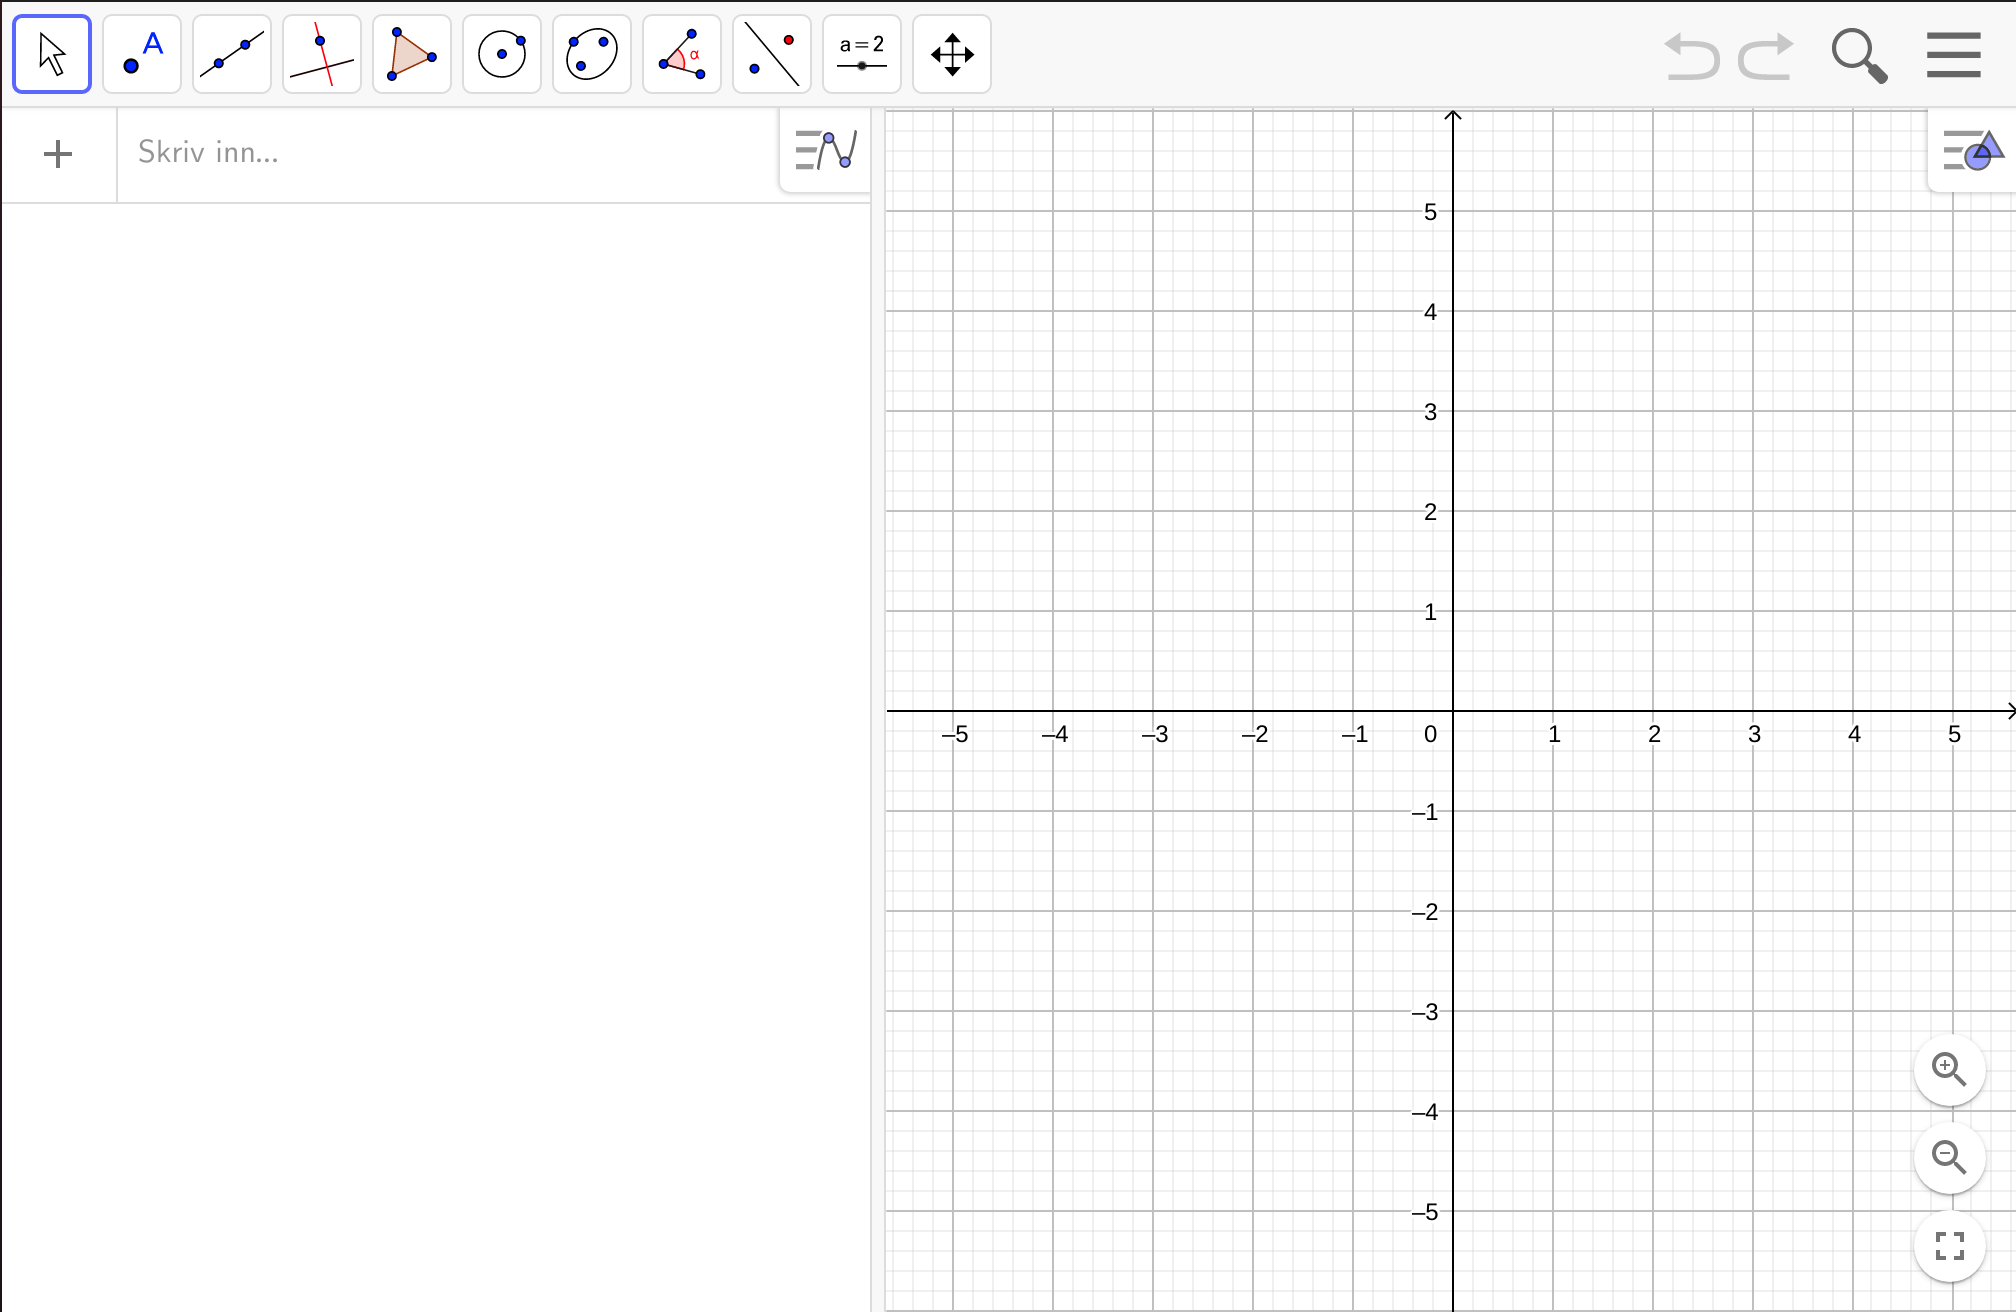
\includegraphics[scale=0.1]{ggbalgoggraf}
\end{figure}
Feltet hvor det står ''Skriv inn'' kalles \textit{inntastingsfeltet}. Dette feltet og det blanke feltet under utgjør \textit{algebrafeltet}. Koordinatsystemet til høyre kalles \textit{grafikkfeltet}.

\subsection{Å skrive inn punkt, funksjoner og linjer}
\subsubsection{Punkt}
Si at vi ønsker å få punktene $ (1,3) $ og $ (4,5) $ til å vises i grafikkfeltet. I inntastingsfeltet skriver vi da
\g{(1,3)}
og \vs
\g{(4,5)}
GeoGebra kaller da punktene $ A $ og $ B $, og tegner dem inn i grafikfeltet:
\begin{figure}[H]
	\centering
	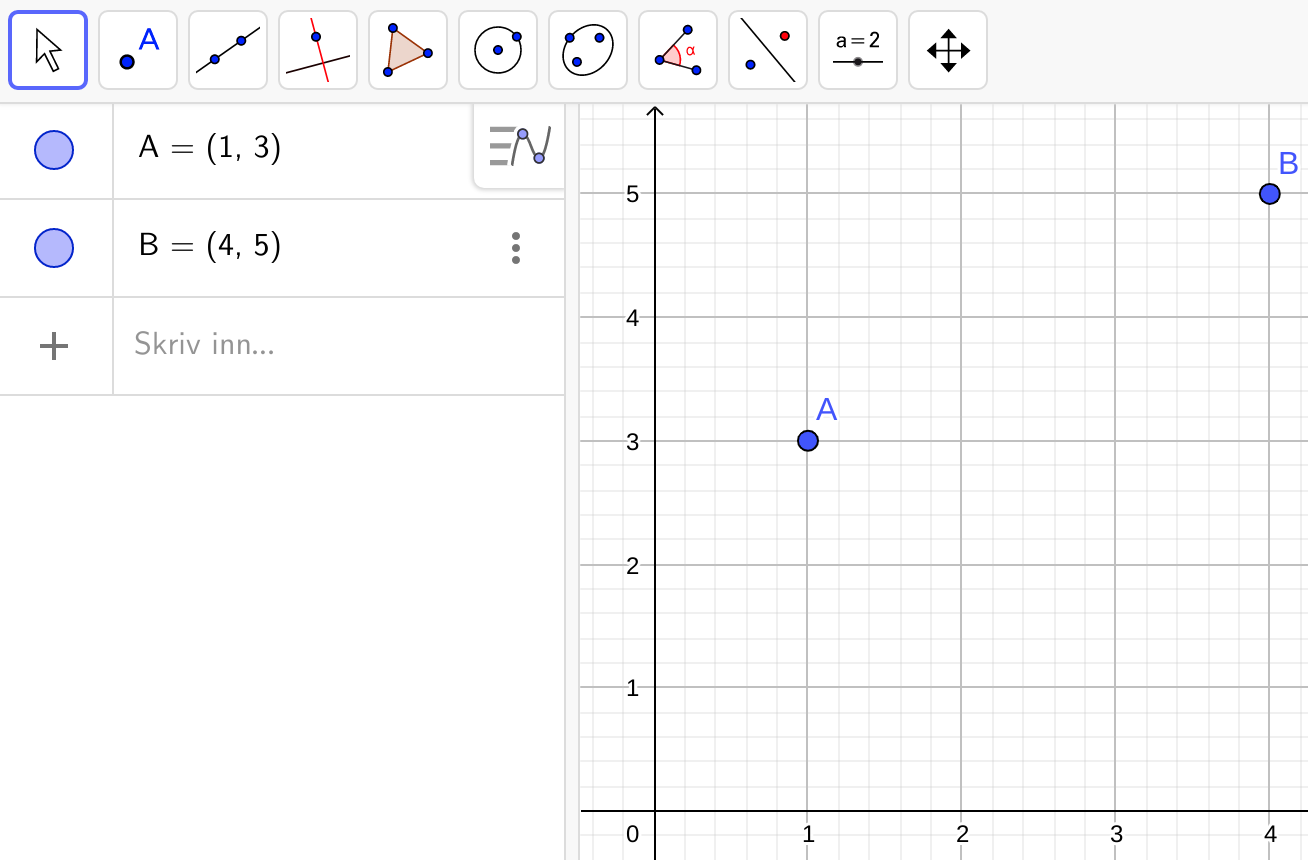
\includegraphics[scale=0.15]{pointAandB}
\end{figure}
Ønsker vi å selv et punkts navn kan vi f. eks skrive
\g{P=(2,4)}
\begin{figure}[H]
	\centering
	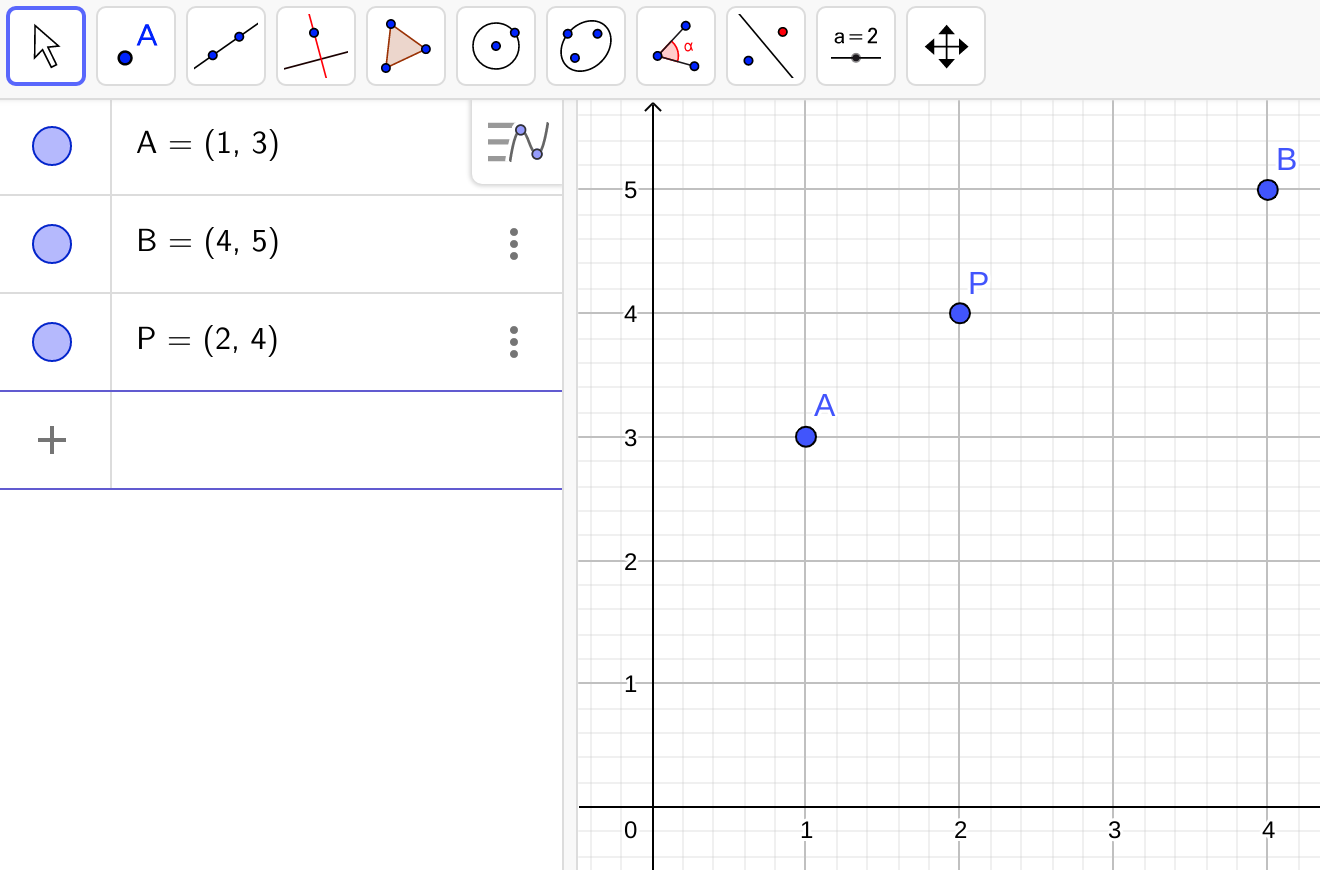
\includegraphics[scale=0.15]{pointP}
\end{figure}
\subsubsection{Funksjoner}
Si vi har funksjonen 
\[f(x)= \frac{3}{2} x^2 + 3x \]
For å bruke $ f(x) $ i GeoGebra, skriver vi:
\g{3/2*x\^{}2+3x}
Når vi ikke gir funksjonen noen navn, vil GeoGebra automatisk gi funksjonen navnet $ f $. I algebrafeltet får vi derfor
\begin{figure}[H]
	\centering
	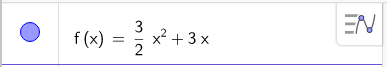
\includegraphics[scale=0.5]{skrivf}
\end{figure}
I grafikkfeltet får vi grafen til $ f $. \vsk

Hvis vi isteden har funksjonen
\[ P(x)= 0,15x^3 - 0,4 x\]
er det to ting vi må passe på. Det første er at \textsl{alle desimaltall må skrives med punktum istedenfor komma} i GeoGebra
. Det andre er at vi ønsker å gi funksjonen navnet $ P(x) $. Vi skriver da
\g{P(x) = 0.15x\^{}3 - 0.4x}
og får \vspace{-5pt}
\begin{figure}[H]
	\centering
	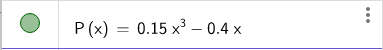
\includegraphics[scale=0.5]{pfig}
\end{figure}
\info{Obs!}{
Man kan aldri gi funksjoner navnet $ {y(x)} $ i GeoGebra. $ y $ kan bare brukes når man skriver inn uttrykk for en rett linje, altså $ {y=ax +b} $, hvor $ a $ og $ b $ er to valgfrie tall.
}

\subsubsection{Vannette og loddrette linjer}

Ønser vi å lage ei linje som går vannrett gjennom verdien 3 på $ y $-aksen og ei linje som går loddrett gjennom verdien 2 på $ x $-aksen skriver vi:
\g{y = 3}
og 
\g{x = 2 }
Da får vi denne figuren:
\begin{figure}[H]
	\centering
	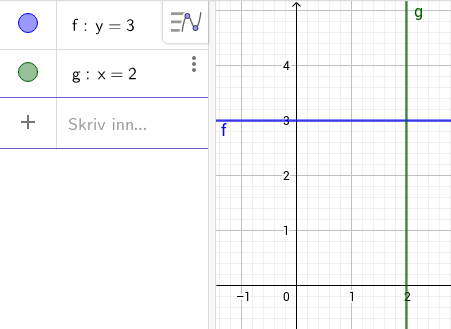
\includegraphics[scale=0.5]{23}
\end{figure}

\subsection{Å finne verdien til funksjoner og linjer}
\subsubsection{Funksjoner}
Si vi har funksjonen
\[H(x)= x^2 + 3x -3 \]
Hvis vi ønsker å vite hva $ H(2) $ er, skriver vi
\g{H(2)}
som resulterer i dette
\begin{figure}[H]
	\centering
	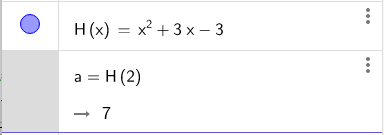
\includegraphics[scale=0.5]{H}
\end{figure}
Da vet vi at $ H(2)=7 $.
\subsubsection{Linjer}
Det anbefales på det sterkeste at du bruker funksjonsuttrykk når du behandler linjer i GeoGebra, men i noen tilfeller kommer man ikke utenom linjer på former $ y=ax+b $. \vsk

La oss se på de to linjene \vs
\alg{
	y&= x-3 \vn
	y&= -2x+1
}
Vi skriver disse inn i GeoGebra, og får
\begin{figure}[H]
	\centering
	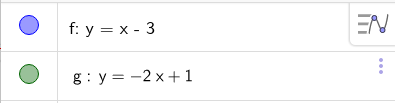
\includegraphics[scale=0.5]{fglin1}
\end{figure}
Ønsker vi nå å finne hva verdien til $ {y=x-3} $ er når $ {x=2} $, må vi legge merke til at GeoGebra har kalt denne linja for $ f $. Svaret vi søker får vi da ved å skrive $ f(2) $. Ønsker vi samtidig å vite hva $ {y=-2x+1} $ er når $ {x=0} $, må vi skrive $ g(0) $:
\begin{figure}[H]
	\centering
	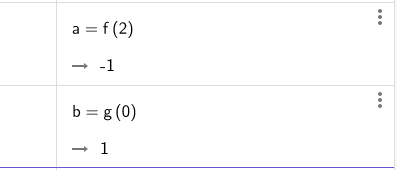
\includegraphics[scale=0.6]{fglin2}
\end{figure}

\newpage
\subsection{Knapper og kommandoer}

\subsubsection*{Grafikkfelt}
Knappene velges fra rullemenyer på verktøylinjen. Nummereringen av menyene er fra venstre.\vsk

\begin{tabular}{@{}l}
	\,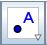
\includegraphics[scale=0.4]{fig/pkt} Lager et nytt punkt. (Meny nr. 1) \\
	\,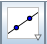
\includegraphics[scale=0.4]{fig/lin} Lager linje mellom to punkt. (Meny nr. 2)\\	
	\,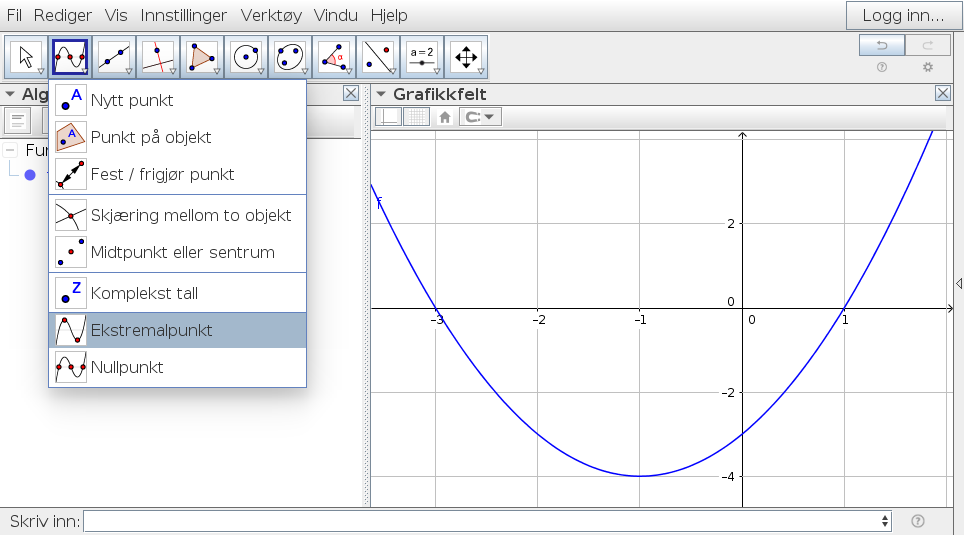
\includegraphics[scale=0.4]{fig/ekst} Finner topp- og bunnpunkt til en funksjon. (Meny nr. 2)\\
	\,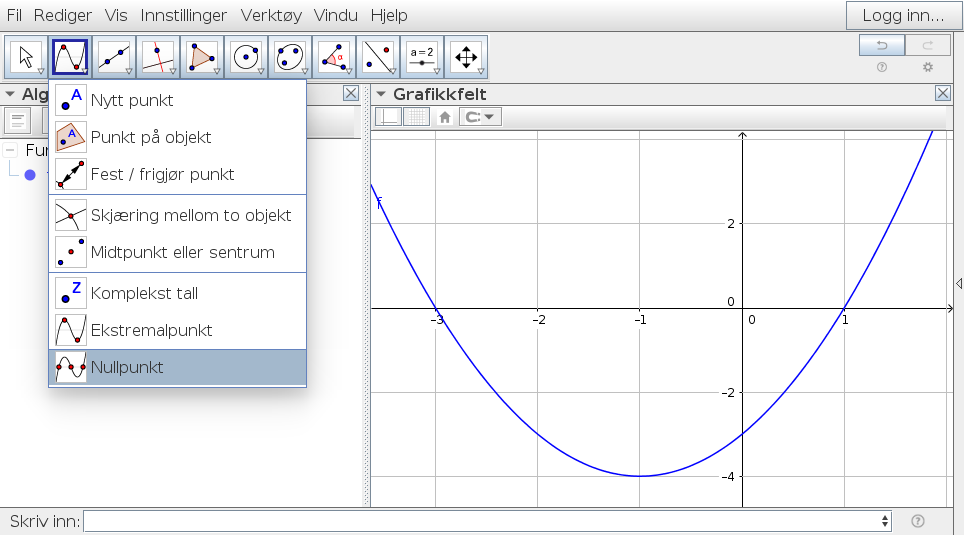
\includegraphics[scale=0.4]{fig/nul} Finner nullpunktene til en funksjon. (Meny nr. 2)	\\
	\,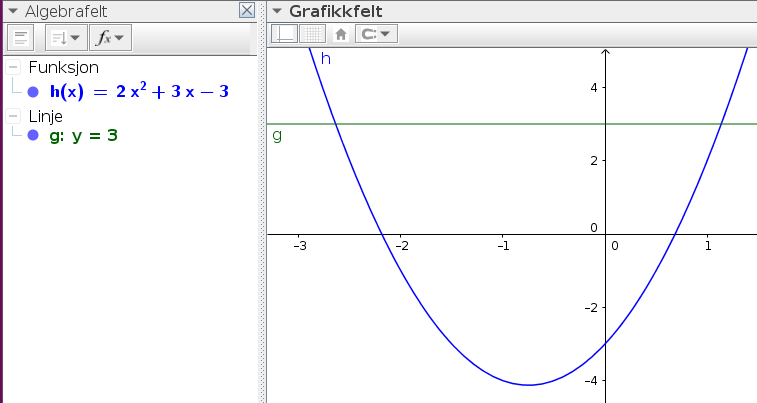
\includegraphics[scale=0.4]{fig/skj} Finner skjæringspunkt mellom to objekt. (Meny nr. 3)\\	
	\,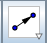
\includegraphics[scale=0.4]{fig/vek} Lager vektoren mellom to punkt (Meny nr. 3)\\		
	\,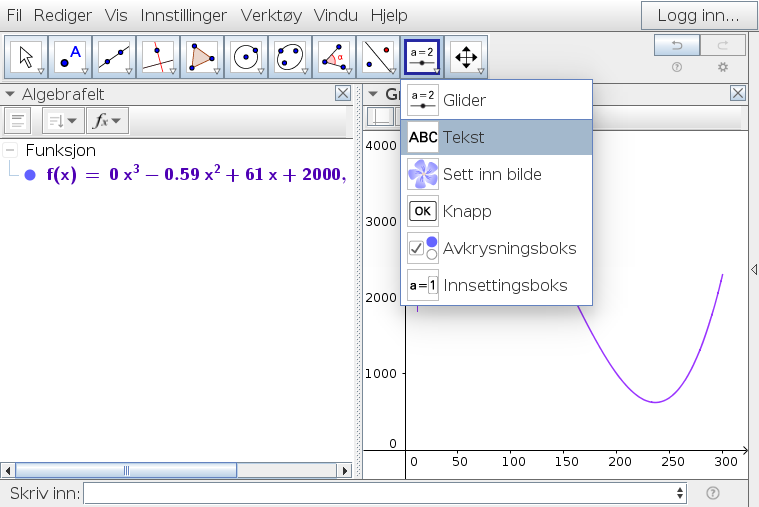
\includegraphics[scale=0.4]{fig/tekst} Lager en tekstboks. (Meny nr. 10)\\		
	\,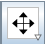
\includegraphics[scale=0.4]{fig/flytt} Flytter grafikkfeltet. Endrer verdiavstanden hvis man peker på aksene. \\
	\hspace{1cm}(Meny nr. 10)\\			
\end{tabular}

\subsubsection{Hurtigtaster}
\begin{tabular}{@{}c | c |c | c }
	&\textbf{Beskrivelse} & \textbf{PC }& \textbf{Mac} \\ \hline
	$ \sqrt{} $	& kvadratrot& \texttt{alt\,+\,r} &\texttt{alt\,+\,r} \\\hline
	$ \pi $	& pi& \texttt{alt\,+\,p} & \texttt{alt\,+\,p}\\\hline
	$ \infty $ &uendelig& \texttt{alt\,+\,u} &\texttt{alt\,+\,,}  \\\hline
	$ \otimes $&kryssprodukt & \texttt{alt\,+\,shift\,+\,8}&\texttt{ctrl\,+\,shift\,+\,8} \\\hline
	$ e $&eulers tall & \texttt{alt\,+\,e}& \texttt{alt\,+\,e}\\\hline
	$ {}^\circ $&gradtegnet ($ \frac{\pi}{180} $) & \texttt{alt\,+\,o}& \texttt{alt\,+\,o}
	\\\hline	
\end{tabular}
\newpage
\subsubsection{Videoer}
\begin{itemize}
\item \net{https://drive.google.com/file/d/1u9u6eZFW8yqtM2ukdW9716i1_YH0NMOa/view?usp=sharing}{Finne nullpunktene til en graf}
\item \net{https://drive.google.com/file/d/11B7o3WMrbR5cpfshkv9FSBpQ5khBCwLS/view?usp=sharing}{Finne lokale bunnpunkt (eller toppunkt) til en graf}
\item \net{https://drive.google.com/file/d/1koy-ffEejtIt-YbIohoFN4gbMLi-95cb/view?usp=sharing}{Finne skjæringspunktene til to funksjoner}
\item \net{https://drive.google.com/file/d/1Z8v05XjlqsSFpHEed5q4s0nGDjdQUfqs/view?usp=sharing}{Justere akser}
\item \net{https://drive.google.com/file/d/1oKKDk084IEhy11rNhDk0-VykzXLuhthy/view?usp=sharing}{Endre tykkelse, farge o.l på graf}
\item \net{https://drive.google.com/file/d/1568rRj2PxzwK6wSm7v4w3GWzDnGtSuuX/view?usp=sharing}{Tegne graf på gitt intervall}	\\
{\footnotesize I videoen tegner vi $f(x)= x^2-3x+2 $ på intervallet $ 0\leq x \leq 5 $}.
\item \net{https://drive.google.com/file/d/1x7y7DJMJ-7rfpgapB48e5Nlq6UnXXcI2/view?usp=sharing}{Lage linje mellom to punkt}	\\
{\footnotesize Legg merke til hva som gjøres mot slutten av videoen for å få det vante uttrykket $ y=ax+b $}.
\item \net{https://drive.google.com/file/d/18cNeX3vJFEY7BpgrH_BFpI1q4c-bczyH/view?usp=sharing}{Utføre regresjon i algebrafelt}\\
{\footnotesize I videoen har vi på forhånd skrevet inn tallene i tabellen under, som viser elbilsalget i Norge antall år etter 2010. Disse tallene ble også brukt i \refsec{Regresjon}. \os
Det utføres regresjon med en linje, en kvadratisk funksjon og en 4. grads funksjon.
	
\begin{tabular}{c|c}
	\textbf{antall år} & \textbf{elbiler} \\ \hline
	0 &	3347\\
	1 &	5381\\
	2 &	9565\\
	3 &	19678\\
	4 &	42356\\
	5 &	73312\\
	6 &	101126\\
	7 &	138477\\
	8 &	194900\\
	9 &	260688\\
	10 &337201\\
	11 &	455271\\
\end{tabular}
}
\item \net{https://drive.google.com/file/d/1GYSaDyHt064yqmCBpfmbJATRDs6aWuBP/view?usp=sharing}{Regresjonsanalyse i regnearket}\\
{\footnotesize I videoen finner vi hvilket polynom som best beskriver summen av de $ n $ første kvadrattallene ($ 1^2 $, $ 2^2 $, $ 3^2 $ og så videre). $ R^2 $ er et tall mellom 0 og 1 som viser hvor nærme funksjonen er å skjære gjennom hvert punkt, hvor $ R^2=1 $ betyr at funksjonen skjærer hvert punkt eksakt. 
\begin{center}
	\begin{tabular}{c|c}
	\boldmath $ n $ & \textbf{sum}\\
	1 & 1\\
	2 & 5\\
	3 & 14 \\
	4 & 30 \\
	5 & 55	
\end{tabular}
\end{center}
}




\end{itemize}
\newpage
\subsubsection{Kommandoliste}
\mers{Mange av kommandoene har egne knapper, som blant annet vist i videoene over.}
\begin{itemize}
	\item \cmds{abs( <x> )}{Gir lengden til $ x $ (et tall, et linjestykke o.l.). Alternativt kan man skrive {\tt{|x|}}}.
	
	\item \cmds{Linje( <Punkt>, <Punkt> )}{Gir linjen mellom to punkt.}
	
	\item \cmds{Ekstremalpunkt( <Funksjon>, <Start>, <Slutt> )}{Finner lokale topp- og bunnpunkt for en funksjon på et gitt intervall.}
	
	\item \cmds{Funksjon( <Funksjon>, <Start>, <Slutt> )}{Tegner en funksjon innenfor et gitt intervall.}
	
	\item \cmds{Mangekant( <Punkt>, ..., <Punkt> )}{Tegner mangekanten mellom gitte punkt.}
	
	\item \cmds{Nullpunkt( <Funksjon>, <Start>, <Slutt> )}{Gir nullpunktene til en funksjon innenfor et gitt intervall}
	
	\item \cmds{RegLin( <Liste> )}
	{Bruker regresjon med en rett linje for å tilpasse punkt gitt i en liste.}
	
	\item \cmds{RegEksp( <Liste> )}
	{Bruker regresjon med en eksponentialfunksjon for å tilpasse punkt gitt i en liste.}
	
	\item \cmds{RegPoly( <Liste>, <Grad> )}
	{Bruker regresjon med et polynom av gitt grad for å tilpasse punkt gitt i en liste.}
	
	\item \cmds{RegPot( <Liste> )}
	{Bruker regresjon med en potensfunksjon for å tilpasse punkt gitt i en liste.}
	
	\item \cmds{Skjæring( <Objekt>, <Objekt> )}{Finner skjæringspunktene til to objekt (funksjoner, linjer o.l.)}
	
\end{itemize}



\end{document}

